\documentclass[12pt,a4paper]{article}
\usepackage{fullpage}
\usepackage[margin=2cm]{geometry}
\usepackage{amsmath}
\usepackage{subfig}
\usepackage{graphicx}
\begin{document}
\title{Local features and landmarks identification}
\author{LE Van Linh and BEURTON-AIMAR Marie}
\date{May, 2017}
\maketitle
\begin{abstract}

	In this work, we study the local features on the image and the integration among the features. Besides, we used some of the local features to try for estimating the landmark on the "pronotum". The results show evaluation on the integration between them and the proportion of the landmark on the "pronotum".

\end{abstract}
\section{Introduction}
The image features are the characteristics of the image (such as color, magnitude, direction,...) that used as the input of the image processing technique. Based on the way to consider the characteristics of the image, the features can be divided into two classes: global features and local features. The term "global" is aimed when we consider whole the image. It is used in contours detection \cite{canny1986computational, smith1997susan}, shape descriptors[cite], object recognition[cite]. While, the "local" feature describes the feature in a small patch in the image, usual the neighbourhood of a pixel \cite{lowe2004distinctive}. The local feature is more used in the texture representation.

In this part, we introduce some local features which have used in recent years and the integration between them. Besides, some evaluation is shown and using them to determine the landmark on the pronotum.

\section{Local features}

\subsection{Image gradient}
The simplest feature can be used as the local feature is image gradient. It is computed directly from the intensity or color of the image. Because the image is composed of the discrete pixels, so the gradient of a pixel can be computed as approximation of its value and the neighbourhood value. The common way to calculate the image gradient is convolve the image with an kernel, such as Gaussian operator \cite{maini2009study}, Robert operator \cite{maini2009study}, Sobel operator \cite{maini2009study} or Prewitt operator\cite{maini2009study}. The gradient feature have been used to detect the contour\cite{canny1986computational}, corner \cite{smith1997susan}, point of interest \cite{lowe2004distinctive}.

When talk about the gradient of the image, we usually ear to the magnitude and direction of the gradient which given by the formula:
\begin{equation}
	\nabla f = \begin{bmatrix}
					g_x \\
					g_y
				\end{bmatrix},  
\end{equation}
\begin{equation}
	\theta = tan^{-1}(\frac{g_y}{g_x})
\end{equation}
Where: 
\begin{itemize}
	\item $g_x$: is the gradient in x direction
	\item $g_y$: is the gradient in y direction
	\item $\nabla f$: is the gradient magnitude
	\item $\theta$: is the gradient direction
\end{itemize}
\subsection{Local binary pattern}
Local Binary Pattern (LBP) is a model of texture analysis based on the texture unit (a small patch of the image). It is introduced the first time by Wang and He \cite{wang1990texture} with 6561 possible texture units in a $3 \times 3$ patch. Timo Ojala et al \cite{ojala1996comparative} proposed another level (two-level) for the texture descriptor, there are only $2^8 = 256$ possible texture units instead of 6561. In the binary case, the elements in $3 \times 3$ patch are thresholded by the value of center pixel. A weight patch corresponding with the patch is created. The value at each position in weight patch is exponential of two following the clockwise direction or counter-clockwise direction. The value of the pixels in the thresholded patch are multiplied with the corresponding pixels in weight patch. Finally, the value of eight pixels are summed to obtain the LBP value of the texture unit. The LBP method is a gray-scale invariant and it can be easily combined with other features to use in the application of texture.
\subsection{Contrast}
Contrast is the difference in luminance or color that make the object distinguishable. Depend on the situations of using, the definitions of contrast are defined in different.\\
\textit{Weber} \cite{fechner1948elements} defines contrast as (equation \ref{webercontrast}):
\begin{equation}
	C = \frac{I - I_b}{I_b}
	\label{webercontrast}
\end{equation}
Where:
\begin{itemize}
	\item  $C$: is the contrast of the image,
	\item  $I, I_b$: are luminance of the features and the background, respectively.
\end{itemize}
\textit{Michelson} \cite{michelson1995studies} use the highest ($I_{max}$) and lowest ($I_{min}$) luminance to calculate the contrast (equation \ref{michelsoncontrast}). This calculation is commonly used for patterns.
\begin{equation}
	C = \frac{I_{max} - I_{min}}{I_{max} + I_{min}}
	\label{michelsoncontrast}
\end{equation}
The Root Mean Square (RMS) \cite{peli1990contrast} contrast is defined as the standard deviation of pixel intensities: 
\begin{equation}
	C = \sqrt{\frac{1}{MN}\sum_{i=0}^{N-1}\sum_{j=0}^{M-1}(I_{ij} - \overline{I})^2}
\end{equation}
Where:
\begin{itemize}
	\item  $C$: is the contrast of the image,
	\item $M,N$: are the size of the image
	\item $I_{ij}$: is intensity at position $(i,j)$.
	\item $\overline{I}$: is the average intensity of all pixel values in the image
\end{itemize}
\subsection{Center-symmetric covariance measures}
SCOV is a measure of the pattern correlation. It was introduced by David Harwood et al \cite{•}. It measures covariance of any local center-symmetric pattern. The measure is abstract measures of texture pattern and grey-scale, providing the discriminating information about the amount of local texture. The SCOV of a $3 \times 3$ neighbourhood (see fig \ref{figscov}) for center-symmetric pairs of the pixels are calculated by the equation (\ref{scov}):
\begin{figure}[htb]
    \centering
    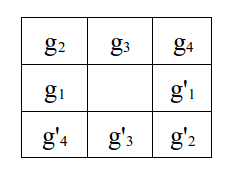
\includegraphics[width=0.2\textwidth]{./images/scov}
    \caption{A $3 \times 3$ neighborhood for center-symmetric pairs.}
    \label{figscov}
\end{figure}
\begin{equation}
	SCOV = \frac{1}{4}\sum_i^{4}(g_i - \mu)(g_i' - \mu)
	\label{scov}
\end{equation} 
Where: 
\begin{itemize}
	\item $g_i$: is grey-level of pixel $i$
	\item $g'_i$: is the grey-level of pixel that symmetric with pixel $i$
	\item $\mu$: is the local mean
\end{itemize}
\section{Features integration}
In most case, a single texture feature is not enough information to present for amount and spatial of local texture. The better way is considering the combination between two or more features. As an example, Lowe \cite{lowe2004distinctive} considered the use of gradient magnitude and direction to detect the dominant point in the image; Timo Ojala et al \cite{ojala1996comparative, ojala1999unsupervised} used LBP/Contrast and LBP/SCOV to classify the texture in the image.
\section{Local features and landmark estimation}
In this section, we show a way to combine the local features and evaluate the correctness of them for estimating the landmark on beetle's pronotum. Local binary pattern (LBP) and contrast(C) have been selected.\\
By using two images (source and target image) and their manual landmarks, method shows the way to evaluate the landmarks on the others. It includes two steps: (1) create the texture descriptor; (2) compare the similarity among the descriptors. Each landmark of the source image will be evaluated with all the landmarks of the target image.

For each manual landmark, a patch centered at the landmark is created  with size $s$. Then, for each pixel in the patch, a $3 \times 3$ neighborhood (Fig. \ref{figlbpc}a) is used to calculate the LBP and contrast. The original $3 \times 3$ patch is thresholded by the value of the center pixel (Fig. \ref{figlbpc}b). The values of the pixels in the thresholded neighborhood are multiplied by the binomial weights given to the corresponding pixels(Fig. \ref{figlbpc}c). The LBP of texture unit is summed of all obtained values (Fig. \ref{figlbpc}d). The contrast of the texture unit is defined as the difference between the average gray-level of the 1-pixels and 0-pixels. The contrast then is mapped from the continuous value to the discrete value by quantization. The pair LBP/C after that is presented into a two-dimensional accumulator of size $256 \times b$, where $b$ is number of discrete contrast. The process is continued until all pixels in the patch are considered.\\
\begin{figure}[htb]
    \centering
    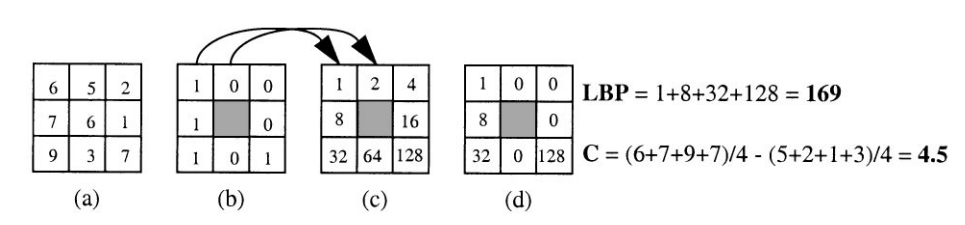
\includegraphics[width=0.9\textwidth]{./images/lbpc}
    \caption{LBP and contrast (C) computing.}
    \label{figlbpc}
\end{figure}
The comparing between the descriptors is done by using $L2$ distance.
\section{Result}
Timo Ojala et al \cite{ojala1999unsupervised} have proposed a method to segment the texture using LBP/C. The evaluation is done on Mosaic \#2 (a $512 \times 512$ image containing four texture made by a GMRF process). The segmentation error is 4.2\% error for the first sweep, it is quite decent. The final error is 1.2\% (after 23 sweeps); Mosaic \#3 (a $512 \times 512$ image with a background made by a GMRF process and four distinct regions) with final error is 1.9\% after 13 sweeps; Mosaic \#4, \#5 are composed of textures taken from outdoor scene. The segmentation errors are 3.3\% and 2.1\%, respectively. From this result, the combining between LBP and contrast could be a good pair for the classification application. An advantage of this method that it does not require any knowledge about how many texture or regions in the image.


In the context of combining the local features, we apply LBP/C to evaluate the effect of this feature pair on the texture around the landmark (as described before). The result shows that the distance of pair at landmark $3^{rd}, 4^{th}, 6^{th}, 7^{th}$ is better than other ones. This mean that the pair LBP/C is worked well on the pattern which have the distinctable pixels.
\section{References}
\bibliographystyle{plain}
\bibliography{includes/localfeatures}
\end{document}